% ----------------------------------------------------------
% FIGURE: RAL UPLIFT TRADEOFF CURVES
% ----------------------------------------------------------
\begin{figure}[htbp]
\centering
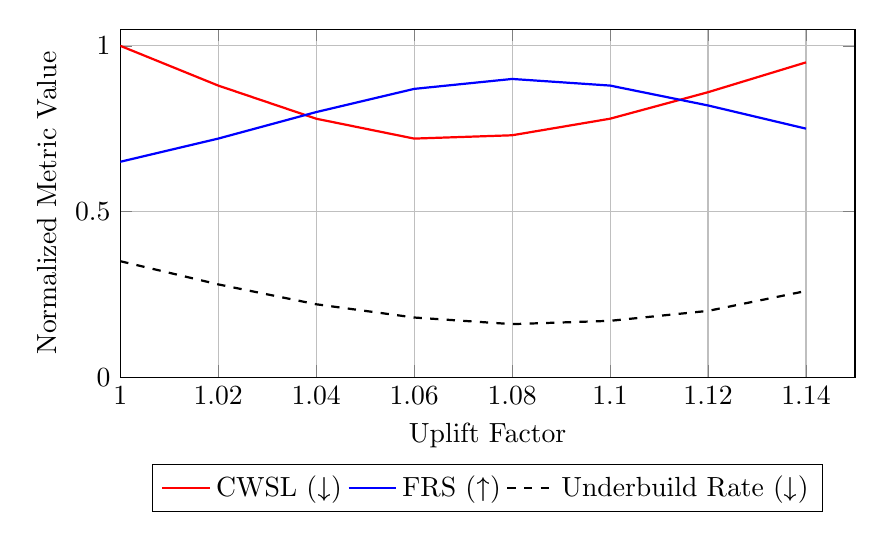
\begin{tikzpicture}
\begin{axis}[
    width=0.9\textwidth,
    height=6cm,
    xlabel={Uplift Factor},
    ylabel={Normalized Metric Value},
    xmin=1.0, xmax=1.15,
    ymin=0, ymax=1.05,
    legend style={at={(0.5,-0.25)}, anchor=north, legend columns=3},
    grid=major,
]

% CWSL (lower is better)
\addplot[thick, red]
coordinates {
    (1.00, 1.00)
    (1.02, 0.88)
    (1.04, 0.78)
    (1.06, 0.72)
    (1.08, 0.73)
    (1.10, 0.78)
    (1.12, 0.86)
    (1.14, 0.95)
};
\addlegendentry{CWSL (↓)}

% FRS (higher is better)
\addplot[thick, blue]
coordinates {
    (1.00, 0.65)
    (1.02, 0.72)
    (1.04, 0.80)
    (1.06, 0.87)
    (1.08, 0.90)
    (1.10, 0.88)
    (1.12, 0.82)
    (1.14, 0.75)
};
\addlegendentry{FRS (↑)}

% Underbuild Rate (lower is better)
\addplot[thick, dashed, black]
coordinates {
    (1.00, 0.35)
    (1.02, 0.28)
    (1.04, 0.22)
    (1.06, 0.18)
    (1.08, 0.16)
    (1.10, 0.17)
    (1.12, 0.20)
    (1.14, 0.26)
};
\addlegendentry{Underbuild Rate (↓)}

\end{axis}
\end{tikzpicture}
\caption{
Illustrative tradeoffs between cost-weighted service loss (CWSL),
Forecast Readiness Score (FRS), and underbuild rate as a function of
the uplift factor within a bounded feasibility envelope.
}
\label{fig:ral_uplift_tradeoff}
\end{figure}